\problem{Show that the locus of poles of the Chebyshev filter is elliptic.}
The transfer function of a chebyshev filter is given as,
\begin{equation}
   |T(j\omega)|^2=\frac{1}{1+\epsilon^2C_n^2(\omega)}
   \label{eqn:chebyshev-tfr1}
\end{equation}
We also have,
\begin{equation}
    |T(j\omega)|^2=T(s)T(-s)|_{s=j\omega}
    \label{eqn:chebyshev-tfr2}
 \end{equation}
Equating Equation~\ref{eqn:chebyshev-tfr1} and Equation~\ref{eqn:chebyshev-tfr2}, we get,
\begin{equation}
    T(s)T(-s)=\ddfrac{1}{1+\epsilon^2C_n^2\left(\frac{s}{j}\right)}
    \label{eqn:chebyshev-tfr-equate}
\end{equation}
The pole locations are calculated by equating the denominator of Equation~\ref{eqn:chebyshev-tfr-equate} as,
\begin{equation}
    \begin{aligned}[b]
        &1+\epsilon^2C_n^2\left(\frac{s}{j}\right)=0\\
        &\Rightarrow \epsilon^2C_n^2\left(\frac{s}{j}\right)=-1\\
        &\Rightarrow C_n^2\left(\frac{s}{j}\right)=\frac{j^2}{\epsilon^2}\\
        &\therefore C_n\left(\frac{s}{j}\right)=\pm \frac{j}{\epsilon}
    \end{aligned}
    \label{eqn:cn-simple}
\end{equation}
For $\omega<<1$, the chebyshev polynomial $C_n(\omega)$ takes the form, $C_n(\omega)=\cos (n \cos^{-1}\omega)$, so, 
\begin{equation}
   \begin{aligned}[b]
    &C_n\left(\frac{s}{j}\right)=\cos\left(n\cos^{-1}\left(\frac{s}{j}\right)\right)
   \end{aligned}
   \label{eqn:cn-complex-1}
\end{equation}
Since $\cos^{-1}\left(\ddfrac{s}{j}\right)$ is a complex number, say,
\begin{equation}
    \cos^{-1}\left(\ddfrac{s}{j}\right)=u+jv
    \label{eqn:ujv}
\end{equation}
From Equation~\ref{eqn:cn-complex-1} and Equation~\ref{eqn:ujv}, we get,
\begin{equation}
    \begin{aligned}[b]
        C_n\left(\frac{s}{j}\right)&=\cos\left(n(u+jv)\right)=\cos\left(nu+jnv)\right)\\
    \therefore C_n\left(\frac{s}{j}\right)&=\cos nu \cosh nv - j \sin nu \sinh nv
    \end{aligned}
    \label{eqn:cn-complex-2}
\end{equation}
Comparing Equation~\ref{eqn:cn-simple} and Equation~\ref{eqn:cn-complex-2}, we get,
\begin{equation}
    \cos nu \cosh nv =0
    \label{eqn:cosn}
\end{equation}

\begin{equation}
    \sin nu \sinh nv=\pm\left(\frac{1}{\epsilon}\right)
    \label{eqn:sinn}
\end{equation}
For Equation~\ref{eqn:cosn} to be true, $\cosh nv\neq0$ since the smallest value it can have is $1$, so, the following must be true.
\begin{equation}
    \begin{aligned}[b]
        &\cos nu = 0\\
        &\Rightarrow u_k = \frac{\pi}{2n} \text{ , } \frac{3\pi}{2n} \text{ , } \frac{5\pi}{2n}\cdots \\
        &\therefore u_k = \frac{(2k-1)\pi}{2n} \quad
        [k=1,2,3,\cdots,n]
    \end{aligned}
    \label{eqn:uk}
\end{equation}
For the value of $u_k$ given by Equation~\ref{eqn:uk}, $\sin nu_k=\pm 1$. So from Equation~\ref{eqn:sinn}, we get,
\begin{equation*}
    \begin{aligned}
        &\sinh nv_k=\pm\left(\frac{1}{\epsilon}\right)\\
        &\Rightarrow nv_k=\sinh^{-1}\left(\pm\frac{1}{\epsilon}\right)\\
        &\therefore v_k=\pm\frac{1}{n}\sinh^{-1}\left(\frac{1}{\epsilon}\right)=\pm a\\
    \end{aligned}
\end{equation*}
Now from Equation~\ref{eqn:ujv} we have,
\begin{equation}
    \begin{aligned}[b]
        &\cos^{-1}\left(\ddfrac{s_k}{j}\right)=u_k+jv_k\\
        &\Rightarrow s_k=j\cos(u_k+jv_k)
        =j\cos\left(\frac{(2k-1)\pi}{2n}\pm j a\right)\\
        &\Rightarrow s_k=j\left[\cos\left(\frac{(2k-1)\pi}{2n}\right)\cosh a \pm j\sin\left(\frac{(2k-1)\pi}{2n}\right)\sinh a \right]\\
        &\therefore s_k=\pm \sin\left(\frac{(2k-1)\pi}{2n}\right)\sinh a + j\cos\left(\frac{(2k-1)\pi}{2n}\right)\cosh a 
    \end{aligned}
    \label{eqn:sk}
\end{equation}
Consider the general equation for $s_k$ as,
\begin{equation}
    s_k=\sigma_k+j\beta_k
    \label{eqn:sk-general}
\end{equation}
Comparing Equation~\ref{eqn:sk} and Equation~\ref{eqn:sk-general}, we get,
\begin{equation}
    \sigma_k=\pm\sin\left(\frac{(2k-1)\pi}{2n}\right)\sinh a 
    \label{eqn:ak-1}
\end{equation}
Considering only negative pole,
\begin{equation}
  \begin{aligned}[b]
    &\sigma_k=-\sin\left(\frac{(2k-1)\pi}{2n}\right)\sinh a \\
    &\therefore \frac{\sigma_k}{\sinh a}=-\sin\left(\frac{(2k-1)\pi}{2n}\right)
  \end{aligned}
    \label{eqn:ak-2}
\end{equation}
\begin{equation}
    \begin{aligned}[b]
       & \beta_k=\cos\left(\frac{(2k-1)\pi}{2n}\right)\cosh a \\
       & \therefore \frac{\beta_k}{\cosh a}=\cos\left(\frac{(2k-1)\pi}{2n}\right)
    \end{aligned}
    \label{eqn:bk}
\end{equation}
Squaring and adding Equation~\ref{eqn:ak-2} and Equation~\ref{eqn:bk}, we get,
\begin{equation}
    \begin{aligned}[b]
        &\left(\frac{\sigma_k}{\sinh a}\right)^2+\left(\frac{\beta_k}{\cosh a}\right)^2=\sin^2\left(\frac{(2k-1)\pi}{2n}\right)
        +\cos^2\left(\frac{(2k-1)\pi}{2n}\right)\\
        &\therefore \left(\frac{\sigma_k}{\sinh a}\right)^2+\left(\frac{\beta_k}{\cosh a}\right)^2=1
    \end{aligned}
    \label{eqn:final}
\end{equation}
Equation~\ref{eqn:final} is an equation for ellipse with,
\begin{equation*}
        \begin{aligned}
        &\text{Major semi-axis}=\cosh a\\
        &\text{Minor semi-axis}=\sinh a\\
        &\text{Focii location}=\pm j
        \end{aligned}
\end{equation*}
\begin{figure}[H]
    \centering
    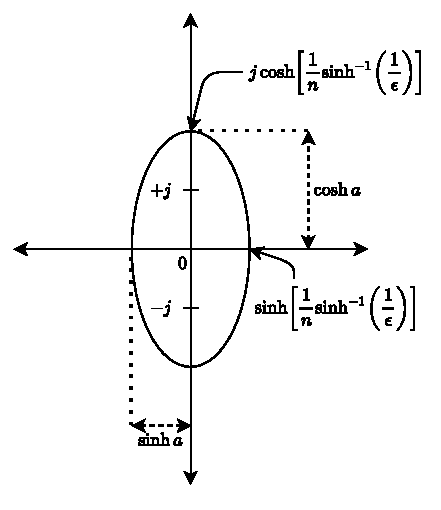
\includegraphics[]{../Figures/pole_location_chebyshev}
    \caption{Pole location for chebyshev lowpass filter}
    \label{fig:chebyshev-pole}
\end{figure}